\documentclass[12pt]{Homework}

% Changed from \usepackage{prelude}
\usepackage{preamble}
\usepackage{amssymb}
\usepackage{enumitem}
\usepackage{mathrsfs}
\def\upint{\mathchoice%
    {\mkern13mu\overline{\vphantom{\intop}\mkern7mu}\mkern-20mu}%
    {\mkern7mu\overline{\vphantom{\intop}\mkern7mu}\mkern-14mu}%
    {\mkern7mu\overline{\vphantom{\intop}\mkern7mu}\mkern-14mu}%
    {\mkern7mu\overline{\vphantom{\intop}\mkern7mu}\mkern-14mu}%
  \int}
\def\lowint{\mkern3mu\underline{\vphantom{\intop}\mkern7mu}\mkern-10mu\int}
\usepackage[mathscr]{euscript}
\usepackage{comment}
\usepackage{MnSymbol}
\usepackage{tikz,float}
\usepackage{tikz-cd}
\usepackage{graphicx}
\usepackage{mathtools}
\usepackage{bbding}
\renewcommand\qedsymbol{\Peace}
\newcommand\placeqed{\nobreak\enspace\Peace}
\usepackage{caption, threeparttable}
\usepackage{halloweenmath}
\newcommand{\contradiction}{\null\hfill\large{$\mathghost$}\normalsize}
\newcommand{\im}{\mathscr{I}\text{m}}
\newcommand{\re}{\mathscr{R}\text{e}}
\newcommand{\res}{\text{Res}}

\name{Kayla Orlinsky}
\course{Complex Analysis Exam}
\term{Spring 2015}
\hwnum{Spring 2015}

\begin{document}

\begin{problem} $\,$
Evaluate the integral $$\int_0^\infty\frac{x^{1/3}}{1+x^2}dx$$ being careful to justify your answer.
\end{problem}


\begin{solution}$\,$
We will use ``Ol' Faithful'' the contour around the upper half plane avoiding the origin since every branch cut of $x^{1/3}=e^{\frac{1}{3}\log x}$ intersects $0$.

Then we take any branch which does not intersect the upper half plane (including the real line).
\begin{center}
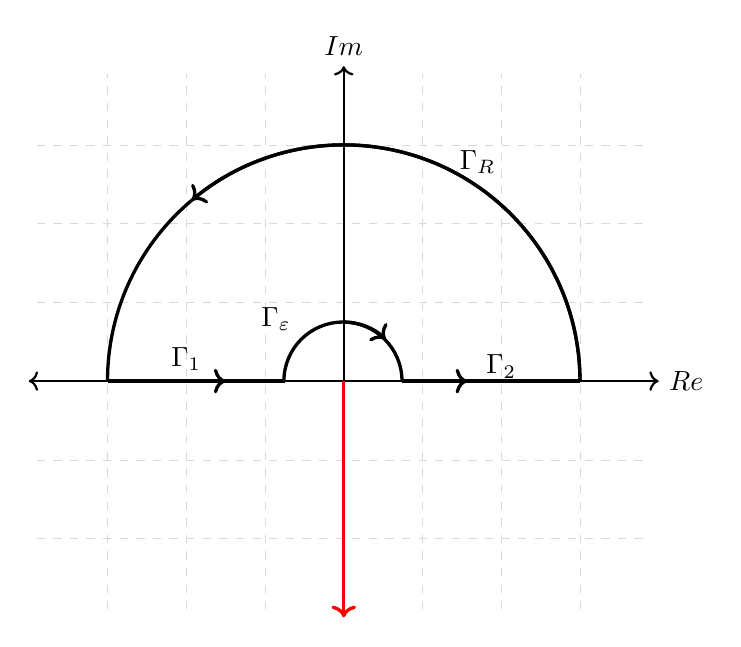
\begin{tikzpicture}
\draw[help lines, color=gray!30, dashed] (-3.9,-2.9) grid (3.9,3.9);
\draw[->,very thick] (3,0) arc (0:130:3cm);
\draw[very thick] (3,0) arc (0:180:3cm) node[above,yshift=2.5cm,xshift=4.7cm]{$\Gamma_R$};
\draw[->,very thick] (0,0.75) arc (90:45:0.75cm);
\draw[very thick] (0.74,0) arc (0:180:0.75cm) node[above,yshift=0.5cm,xshift=-0.1cm]{$\Gamma_\varepsilon$};
\draw[->,very thick] (0.74,0) -- (1.57,0);
\draw[very thick] (0.75,0) -- (3,0) node[above,yshift=-0.1cm,xshift=-1cm]{$\Gamma_2$};
\draw[->,very thick] (-3,0) -- (-1.5,0);
\draw[very thick] (-0.74,0) -- (-3,0) node[above,yshift=0cm,xshift=1cm]{$\Gamma_1$};
\draw[<->, thick] (-4,0)--(4,0) node[right]{$Re$};
\draw[->, thick] (0,0)--(0,4) node[above]{$Im$};
\draw[->,very thick,red] (0,0) -- (0,-3);
\end{tikzpicture}
\end{center}

Let \begin{align*}
    I_1&=\int_{\Gamma_1}\frac{e^{1/3\log z}}{z^2+1}dz\\
    I_2&=\int_{\Gamma_2}\frac{e^{1/3\log z}}{z^2+1}dz\\
    I_\varepsilon&=\int_{\Gamma_\varepsilon}\frac{e^{1/3\log z}}{z^2+1}dz\\
    I_R&=\int_{\Gamma_R}\frac{e^{1/3\log z}}{z^2+1}dz
\end{align*}

Note that \begin{align*}
    I_1&=\int_{\Gamma_1}\frac{e^{1/3\log z}}{z^2+1}dz\\
    &=\int_{-R}^{-\varepsilon}\frac{e^{1/3\log x}}{x^2+1}dx\\
    &=\int_R^\varepsilon\frac{-e^{1/3\log (-x)}}{x^2+1}dx\\
    &=\int_\varepsilon^R\frac{e^{1/3(\log x+i\pi}}{x^2+1}dx\\
    &=e^{i\pi/3}\int_\varepsilon^R\frac{x^{1/3}}{x^2+1}dx\\
    &=e^{i\pi/3}I_2
\end{align*}

Now \begin{align*}
    |I_R|&=\left|\int_{\Gamma_R}\frac{e^{1/3\log z}}{z^2+1}dz\right|\\
    &\le \int_{\Gamma_R}\frac{|e^{1/3\log z}|}{|z^2+1|}d|z|\\
    &\le \int_0^\pi\frac{Re^{1/3\log R}}{R^2-1}d\theta\qquad z=Re^{i\theta}\\
    &=\frac{\pi R^{4/3}}{R^2-1}\to0\qquad R\to\infty
\end{align*}

and \begin{align*}
    |I_\varepsilon|&=\left|\int_{\Gamma_\varepsilon}\frac{e^{1/3\log z}}{z^2+1}dz\right|\\
    &\le \int_{\Gamma_\varepsilon}\frac{|e^{1/3\log z}|}{|z^2+1|}d|z|\\
    &\le \int_\pi^0\frac{\varepsilon e^{1/3\log \varepsilon}}{1-\varepsilon^2}d\theta\qquad z=\varepsilon e^{i\theta}\\
    &=\frac{\pi \varepsilon^{4/3}}{1-\varepsilon^2}\to0\qquad \varepsilon\to0.
\end{align*}

Thus, by the Residue Theorem, \begin{align*}
    2\pi i\res_{z=i}\frac{e^{1/3\log z}}{z^2+1}&=2\pi i\frac{e^{1/3\log (i)}}{i+i}\\
    &=\pi e^{1/3(i\pi/2)}\\
    &=\pi e^{i\pi/6}\\
    &=\lim_{R\to\infty}\lim_{\varepsilon\to0}(I_1+I_2+I_R+I_\varepsilon)\\
    &=(e^{i\pi/3}+1)\int_0^\infty\frac{x^{1/3}}{x^2+1}dx\\
    \implies \int_0^\infty\frac{x^{1/3}}{x^2+1}dx&=\frac{\pi e^{i\pi/6}}{e^{i\pi/3}+1}\\
    &=\frac{\pi}{e^{i\pi/6}+e^{i\pi/6}}\\
    &=\frac{\pi/2}{\cos(\pi/6)}\\
    &=\frac{\pi/2}{\sqrt{3}/2}\\
    &=\frac{\pi}{\sqrt{3}}
\end{align*}
\end{solution}
\newpage



\begin{problem} $\,$
Let $$f(z)=\sum_{n=0}^\infty z^{n!}.$$
\begin{enumerate}[label=(\alph*)]
    \item Show that $f$ is analytic in the open unit disk $D=\{z\in\mathbb{C}:|z|<1\}.$
    \item Show that $f$ can not be analytically continued to any open set properly containing $D.$ (Hint: First consider $z=r^{2\pi ip}/q$ where $p$ and $q$ are integers.
\end{enumerate}
\end{problem}

\begin{solution}$\,$
\begin{enumerate}[label=(\alph*)]
    \item $f$ is holormophic if and only if the sum converges uniformly. For $|z|<r<1$, we have that $|z|^{n!}\le r^{n!}\le r^n$ since $r<1$, and so $f$ converges uniformly by Weierstrass M-test on $\{|z|<r\}.$ Since this holds for all $r<1$, we have that $f$ converges uniformly and is therefore analytic on $D.$
    \item Let $D\subsetneq U$ open. Since $U\not=D$ and $U$ is open, $U$ must contain some $z_0$ with $|z_0|=1.$ 
    
    Again, since $U$ is open, any neighborhood of $z_0$ must contain some $z=e^{i\pi/m}$ for $m\in\mathbb{Z}$ since $|z|=1.$
    
    However, then $$f(z)=\sum_{n=0}^{m-1}e^{in!\pi/m}+\sum_{n=m}^\infty e^{i\pi n!/m}=\sum_{n=0}^{m-1}e^{in!\pi/m}+\sum_{n=m}^\infty 1=\infty$$ since $n!/m\in\mathbb{Z}$ for $n\ge m.$ 
    
    Now, $f$ has a non-removable singularity in every neighborhood of $z_0$.
    
    Namely, $f$ cannot be extended to a neighborhood to $z_0$ since it will not converge in any punctured neighborhood of $z_0.$
\end{enumerate}
\end{solution}
\newpage




\begin{problem} $\,$
Let $A$ be an open subset of $\mathbb{C}$, and suppose $u(x,y)$ is twice continuously differentiable harmonic function on $A.$
\begin{enumerate}[label=(\alph*)]
    \item Show that if $A$ is simply connected, then there exists an analytic function $f$ on $A$ such that $u=\re(f).$ Hint: First find $g$ so that $\partial u/\partial x=\re(g)$).
    \item Find $f$ explicitly when $A=\mathbb{C}$ and $u(x,y)=e^x\cos(y)+xy$.
    \item Give an example in which $A$ is not simply connected and $f$ as in $(a)$ does not exist.
\end{enumerate}
\end{problem}


\begin{solution}$\,$
\begin{enumerate}[label=(\alph*)]
    \item Let $v(x,y)=\int_{y_0}^yu_x(x,t)dt+g(x)-g(x_0).$ Then in order for Cauchy Riemann to be satisfied, \begin{align*}
        -u_y(x,y)&=v_x(x,y)\\
        &=\int_{y_0}^yu_{xx}(x,t)dt+g'(x)\\
        &=\int_{y_0}^y-u_{yy}(x,t)dt+g'(x)\tag{1}\\
        &=-u_y(x,y)+u_y(x,y_0)+g'(x)\\
        \implies -u_y(x,y_0)&=g'(x)\\
        \implies \int_{x_0}^x-u_y(s,y_0)dx&=g(x)-g(x_0)
    \end{align*}
    
    with (1) since $u$ is harmonic so $u_{xx}+u_{yy}=0$.
    
    Therefore, $$v(x,y)=\int_{y_0}^yu_x(x,t)dt-\int_{x_0}^xu_y(s,y_0)dx.$$
    
    Then \begin{align*}
        v_x(x,y)&=\int_{y_0}^yu_{xx}(x,t)dt-u_y(x,y_0)\\
        &=\int_{y_0}^y-u_{yy}(x,t)dt-u_y(x,y_0)\\
        &=-u_y(x,y)+u_y(x,y_0)-u_y(x,y_0)\\\
        &=-u_y(x,y)
    \end{align*}
    
    and $v_y(x,y)=u_x(x,y)$ since $u_y(x,y_0)$ is constant in $y$.
    
    Therefore, $f=u+iv$ is analytic by the Cauchy Riemann with $\re(f)=u$.
    \item Let $u(x,y)=e^x\cos(y)+xy$. Then $$u_y=-e^x\sin(y)+x$$ and so \begin{align*}
        v(x,y)&=-\int u_y(x,y)dx\\
        &=-\int-e^x\sin(y)+xdx\\
        &=-\left(-e^x\sin(y)+\frac{x^2}{2}+h(y)\right)\\
        &=e^x\sin(y)-\frac{x^2}{2}+h(y)
    \end{align*}
    
    Since $$u_x=e^x\cos(y)+y=v_y=e^x\cos(y)+h'(y)\implies h'(y)=y$$ and so $h=\frac{y^2}{2}$ so $$v(x,y)=e^x\sin(y)-\frac{x^2}{2}+\frac{y^2}{2}$$ and $$f(x,y)=e^x\sin(y)+xy+i(e^x\sin(y)-\frac{x^2}{2}+\frac{y^2}{2}).$$
    
    Once can verify that $$u_y=-e^x\sin(y)+x=-(e^x\sin(y)+x)=-v_x$$ and so indeed $f$ is analytic by Cauchy-Riemann.
    \item Let $A=\mathbb{C}\backslash\{0\}$. Then $A$ is not simply connected. Let $u(x,y)=\frac{1}{2}\log(x^2+y^2).$
    
    Then $$u_x=\frac{2x}{2(x^2+y^2)}=\frac{x}{x^2+y^2}$$ and $$u_y=\frac{y}{x^2+y^2}$$
    
    so \begin{align*}
        u_{xx}&=\frac{x^2+y^2-2x^2}{(x^2+y^2)^2}\\
        &=\frac{y^2-x^2}{(x^2+y^2)^2}\\
        &=-\frac{x^2-y^2}{(x^2+y^2)^2}\\
        &=-u_{yy}
    \end{align*} so $u$ is harmonic in $A$.
    
    However, $u$ cannot be the real part of an analytic function, since it is the real part of the complex $\log|z|+iarg(z)$ which is not well defined on $A$. Namely, there is not analytic continuation of $\log z$ (any branch cut) to $A$ and so $u$ cannot be the real part of an analytic function.
\end{enumerate}
\end{solution}
\newpage





\begin{problem} $\,$
Determine whether it is possible for a function $f$ to be analytic in a neighborhood of $0$ and take the values $\frac{1}{2},\frac{1}{2},\frac{1}{4},\frac{1}{4},\frac{1}{6},\frac{1}{6},\frac{1}{8},\frac{1}{8},...$ at the points $1,\frac{1}{2},\frac{1}{3},\frac{1}{4},\frac{1}{5},\frac{1}{6},\frac{1}{7},\frac{1}{8},...$.
\end{problem}


\begin{solution}$\,$
Assume such an $f$ does exist. By continuity, $$\lim_{n\to\infty}f\left(\frac{1}{n}\right)=f(0)=0.$$ Therefore, \begin{align*}
    \lim_{h\to0}\frac{f(h)-f(0)}{h}&=\lim_{n\to\infty}\frac{f\left(\frac{1}{n}\right)}{1/n}\\
    &=\lim_{n\to\infty}\begin{cases}
\frac{1/n}{1/n} & n\text{ even }\\
\frac{1/(n+1)}{1/n} & n\text{ odd }
\end{cases}\\
&=1
\end{align*} so  $f$ is injective in a neighborhood of $0$, which is clearly not true.

Thus, $f$ cannot exist.
\end{solution}


\end{document}
 